\documentclass[a4paper]{article}
\usepackage[14pt]{extsizes}
\usepackage[utf8]{inputenc}
\usepackage[russian]{babel}
\usepackage{vmargin} 
\setmarginsrb{25mm}{25mm}{15mm}{20mm}{0pt}{0mm}{0pt}{0mm}
\usepackage{indentfirst}
\usepackage{graphicx}
\usepackage{amsmath}
\usepackage{amsfonts}

\begin{document}

\begin{titlepage}
    \begin{center}
        \vspace*{\fill}
        {\bfseries Неклассические логики.} \\
        Нечёткая система проветривания помещений.
    \end{center}
    \vspace{\fill}
    \begin{flushright}
        Волокитин Егор \\
        20.Б12 - ПУ
    \end{flushright}
\end{titlepage}

\newpage
\tableofcontents

\newpage
\section{Введение}
В современном мире большое распространение получала концепция 
“домашней автоматизации”, так называемая система “умный дом”. 
Под этими понятиями подразумевают устройства, которые помогают 
человеку выполнять различные повседневные задачи. 

Для примера рассмотрим систему, которая регулирует освещение 
в зависимости от того, насколько много света попадает в помещении 
через окно. Она построена на датчике освещённости, который выведен 
на улицу или к окну. Такое устройство может помогать во время 
работы, поддерживая оптимальную яркость света для глаз, или наоборот, 
готовить ко сну, постепенно приглушая свет. Но не только таким 
образом можно влиять на самочувствие и работоспособность.

На состояние человека сильно влияют таке факторы как температура 
окружающей среды, влажность воздуха и содержание 
углекислого газа в атмосфере. При долгой работе 
в непроветриваемом помещении становится сложнее думать. Для решения 
этой проблемы обычно открывают форточку. В какой-то момент из неё 
начинает сильно дуть, становится холодно, форточку закрывают. 
И так происходит много раз. Почему же не отдать управление проветриванием 
помещения некоторому “умному” устройству.

Такая система поддержания оптимального микроклимата будет иметь в 
основе нечёткое управление, так как такие понятия как температура, 
влажность, спёртость воздуха понимаются всеми людьми по-своему, и очень
сложно понять, при каких точных температуре и влажности надо начинать
проветривание, а при каких его заканчивать.

Основным параметром, который будет регулироваться, является содержание
углекислого газа в помещении, так как он сильнее всего влияет на работу
мозга, и больше всего меняется при проветривании. В целом, можно было бы
постоянно сидеть с открытой форточкой, и содержании углекислого газа всегда
было бы нормальным, но тут начинают играть свою роль температура и
влажность. Изменение этих параметров и заставляет нас закрывать форточку.

Стоит отметить, что измерения будут очень грубыми, так как используются
датчики начального уровня. Но в данном устройстве особая точность не нужна,
в силу специфики нечёткого управления и того, как мы влияем на параметры
системы, а именно регулируем положение окна.

\newpage
\section{Постановка задачи}
Дано окно. Его управлением занимается специальное устройство,  
которое на вход приминиет сообщение о том, в какую позицию надо перевести
окно.

Также даны: цифровой датчик температуры и относительной влажности DHT-11, 
аналоговый датчик газа MQ-135, микроконтроллер atMega328p.

Надо разработать нечёткую систему управления проветриванием помещения,
которая будет считывать значения с датчиков, обрабатывать их, анализировать
и выдавать управляющий сигнал для устройства изменения положения окна.

Система должна стараться поддерживать оптимальные значения влажности,
температуры и содержания углекислого газа в помещении.

Оптимальные значения микроклиматических параметров помещения возьмём из 
{\itshape Санпин 1.2.3685-21} и {\itshape ГОСТ 30494-2011}.

\begin{itemize}
    \item {\bfseries Содержания углекислого газа:} 800 ppm
    \item {\bfseries Температура воздуха:} 22 - 25$^{\circ}$C
    \item {\bfseries Относительная влажность воздуха:} 20 - 70 \%
\end{itemize}

%\newpage
\section{Математическое обоснование}
В 1993 году была доказана Fuzzy Approximation Theorem (FAT), которая
гласит, что любая математическая система может быть аппроксимирована
системой, основанной на начёткой логике. Значит любую систему можно
описать правилами типа 
$$\text{IF \{}x \text{ IS } P(x) \text{\} }\& 
\text{ \{}y \text{ IS } Q(y) \text{\} } 
\rightarrow \text{ \{}z \text{ IS } R(z) \text{\}},$$
где P, Q, R - функции принадлежности, x, y - входные переменные,
z - выходная переменная. Также эти правила формализуются методами 
теории нечётких множеств.

При решении поставленной задачи был использован алгоритм Мамдани,
T-нормой будет функция минимума, композиция будет осуществляться
через max-дизъюнкцию, дефаззификация производится методом центроид.

\newpage
\section{Лингвистические переменные}
На вход системе будет подаваться три переменные:
\begin{itemize}
    \item {\bfseries gas} - cодержания углекислого газа, ppm
    \item {\bfseries temp} - температура воздуха, градусы Цельсия
    \item {\bfseries hum} - относительная влажность воздуха, проценты
\end{itemize}

На выходе системы будет одна переменная:
\begin{itemize}
    \item {\bfseries pos} - в какое положение надо перевести окно 
\end{itemize}

Терм-множества для входных переменных:
\begin{itemize}
    \item {\bfseries T\_gas} = \{norm, stuffy, very stuffy\}
    \item {\bfseries T\_temp} = \{cold, norm, hot\}
    \item {\bfseries T\_hum} = \{dry, norm, wet\}
\end{itemize}

Терм-множество для выходной переменной:
\begin{itemize}
    \item {\bfseries T\_pos} = \{closed, micro, opened, full\} 
\end{itemize}

%\newpage
\section{База правил системы}
{\itshape Правила выведены исходя из экспериментов и здравого смысла.}
\begin{enumerate}
    \item IF \{gas IS norm\} \& \{temp IS cold\} \& \{hum IS dry\} 
        $\rightarrow$ \{pos IS closed\}
    \item IF \{gas IS stuffy\} \& \{temp IS cold\} \& \{hum IS dry\} 
        $\rightarrow$ \{pos IS micro\}
    \item IF \{gas IS very stuffy\} \& \{temp IS cold\} \& \{hum IS dry\} 
    	$\rightarrow$ \{pos IS micro\}
    \item IF \{gas IS norm\} \& \{temp IS norm\} \& \{hum IS dry\} 
    	$\rightarrow$ \{pos IS closed\}
    \item IF \{gas IS stuffy\} \& \{temp IS norm\} \& \{hum IS dry\} 
    	$\rightarrow$ \{pos IS micro\}
    \item IF \{gas IS very stuffy\} \& \{temp IS norm\} \& \{hum IS dry\} 
    	$\rightarrow$ \{pos IS opened\}
    \item IF \{gas IS norm\} \& \{temp IS hot\} \& \{hum IS dry\} 
    	$\rightarrow$ \{pos IS opened\}
    \item IF \{gas IS stuffy\} \& \{temp IS hot\} \& \{hum IS dry\} 
    	$\rightarrow$ \{pos IS opened\}
    \item IF \{gas IS very stuffy\} \& \{temp IS hot\} \& \{hum IS dry\} 
    	$\rightarrow$ \{pos IS full\}
    \item IF \{gas IS norm\} \& \{temp IS cold\} \& \{hum IS norm\} 
    	$\rightarrow$ \{pos IS closed\}
    \item IF \{gas IS stuffy\} \& \{temp IS cold\} \& \{hum IS norm\} 
    	$\rightarrow$ \{pos IS micro\}
    \item IF \{gas IS very stuffy\} \& \{temp IS cold\} \& \{hum IS norm\} 
    	$\rightarrow$ \{pos IS opened\}
    \item IF \{gas IS norm\} \& \{temp IS norm\} \& \{hum IS norm\} 
    	$\rightarrow$ \{pos IS closed\}
    \item IF \{gas IS stuffy\} \& \{temp IS norm\} \& \{hum IS norm\} 
    	$\rightarrow$ \{pos IS opened\}
    \item IF \{gas IS very stuffy\} \& \{temp IS norm\} \& \{hum IS norm\} 
    	$\rightarrow$ \{pos IS full\}
    \item IF \{gas IS norm\} \& \{temp IS hot\} \& \{hum IS norm\} 
    	$\rightarrow$ \{pos IS opened\}
    \item IF \{gas IS stuffy\} \& \{temp IS hot\} \& \{hum IS norm\} 
    	$\rightarrow$ \{pos IS full\}
    \item IF \{gas IS very stuffy\} \& \{temp IS hot\} \& \{hum IS norm\} 
	    $\rightarrow$ \{pos IS full\}
    \item IF \{gas IS norm\} \& \{temp IS cold\} \& \{hum IS wet\} 
    	$\rightarrow$ \{pos IS closed\}
    \item IF \{gas IS stuffy\} \& \{temp IS cold\} \& \{hum IS wet\} 
	    $\rightarrow$ \{pos IS micro\}
    \item IF \{gas IS very stuffy\} \& \{temp IS cold\} \& \{hum IS wet\} 
    	$\rightarrow$ \{pos IS micro\}
    \item IF \{gas IS norm\} \& \{temp IS norm\} \& \{hum IS wet\} 
	    $\rightarrow$ \{pos IS micro\}
    \item IF \{gas IS stuffy\} \& \{temp IS norm\} \& \{hum IS wet\} 
    	$\rightarrow$ \{pos IS opened\}
    \item IF \{gas IS very stuffy\} \& \{temp IS norm\} \& \{hum IS wet\} 
	    $\rightarrow$ \{pos IS full\}
    \item IF \{gas IS norm\} \& \{temp IS hot\} \& \{hum IS wet\} 
	    $\rightarrow$ \{pos IS opened\}
    \item IF \{gas IS stuffy\} \& \{temp IS hot\} \& \{hum IS wet\} 
    	$\rightarrow$ \{pos IS full\}
    \item IF \{gas IS very stuffy\} \& \{temp IS hot\} \& \{hum IS wet\} 
        $\rightarrow$ \{pos IS full\}
\end{enumerate}

%\newpage
\section{Фаззификация переменных}
Для системы были выбраны функции принадлежности, которые соответствуют
графикам на рис. 1 и рис. 2. Такой выбор обоснован тем, что изменение
данных физических параметров происходит плавно, без резких скачков, поэтому
в основном были использованы функции Гаусса. 

\begin{figure}[h]
    \center{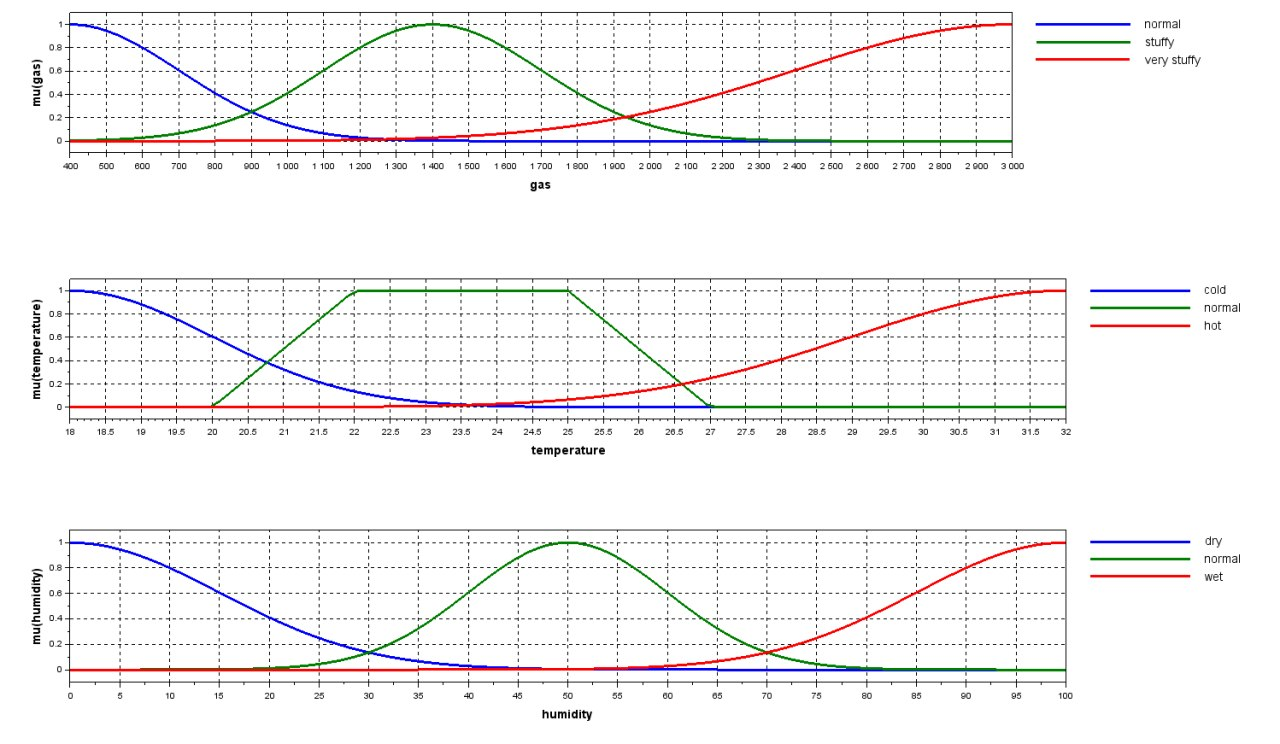
\includegraphics[width=0.7\linewidth]{pics/input_pic}}
    \caption{Функиции принадлежности для входных переменных} 
\end{figure}

\begin{figure}[h]
    \center{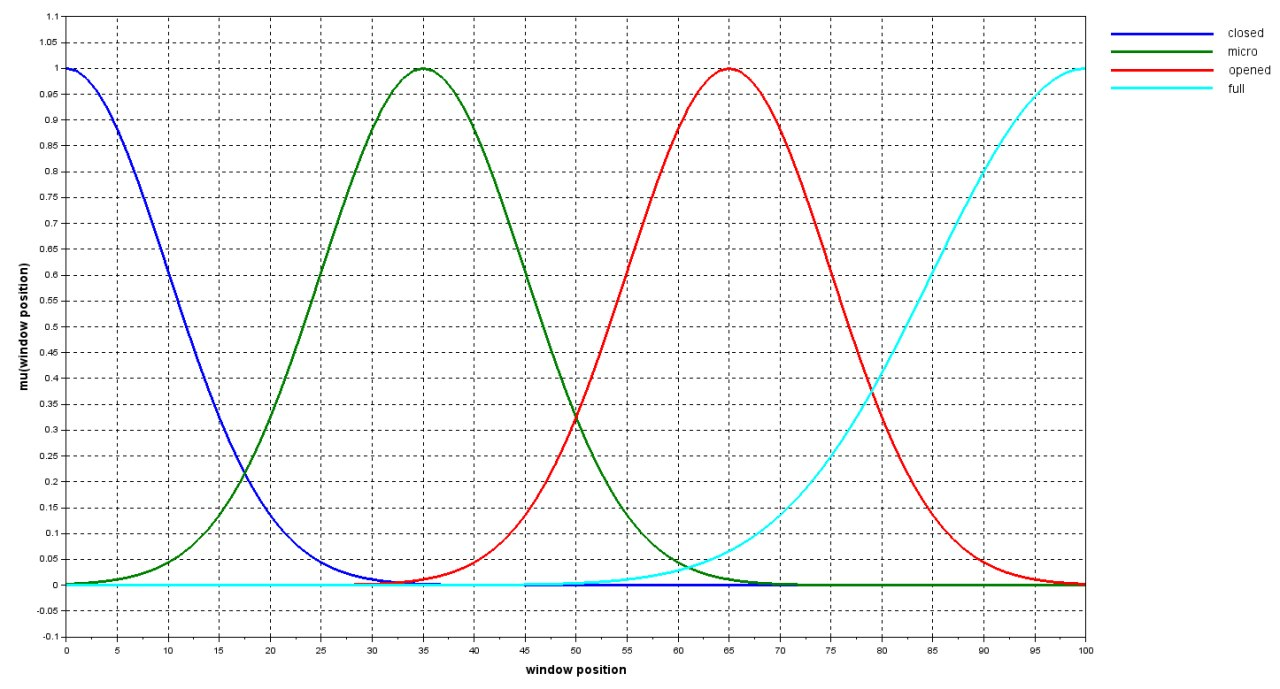
\includegraphics[width=0.7\linewidth]{pics/output_pic}}
    \caption{Функиции принадлежности для выходной переменной} 
\end{figure}

Стоит отметить, что вычислять функцию Гаусса затратнее, чем треугольную или
трапецивидную, и это может сказаться на скорости работы программы
микроконтроллера. Но в нашем случае параметры меняются не очень быстро,
опрос датчиков происходит раз в секунду, и в целом система очень инертна.
Поэтому мы можем тратить время на долгое вычисление действий с числами с
плавающей точкой.

\section{SciLab и sciFLT}
Построение данной системы производилось с помощью программы SciLab и пакета
нечёткой логики sciFLT.

Сначала были заданы основные параметры системы, алгоритм решения и
соответствующие нормы и методы (рис. 3).

Далее в систему были загружены входные и выходные переменные, а также
функции их принадлежности (рис. 4). 

Потом были заданы правила, по которым работает система (раздел 5).


\begin{figure}[h]
    \center{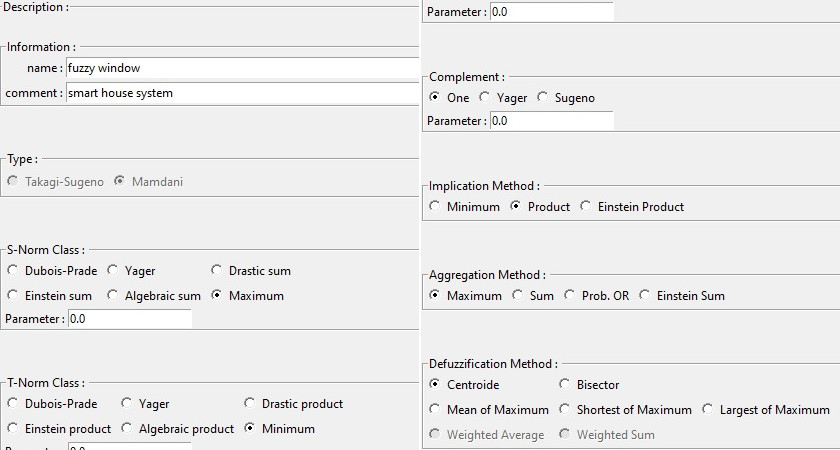
\includegraphics[width=1\linewidth]{pics/info/info}}
    \caption{Параметры SciLab} 
\end{figure}

\begin{figure}[h!]
    \begin{minipage}[h]{0.5\linewidth}
        \center{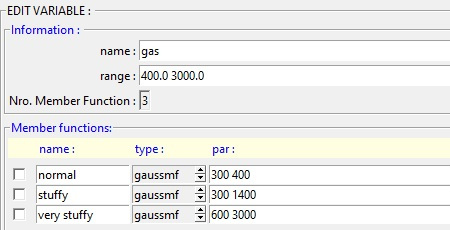
\includegraphics[width=1\linewidth]{pics/info/gas_info}}
    \end{minipage}
    \begin{minipage}[h]{0.5\linewidth}
        \center{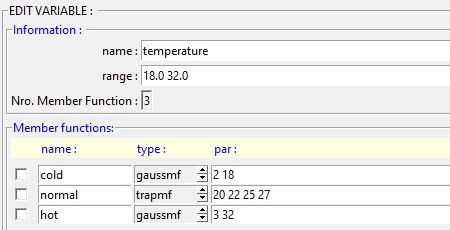
\includegraphics[width=1\linewidth]{pics/info/temp_info}}
    \end{minipage}
    \vfill
    \begin{minipage}[h]{0.5\linewidth}
        \center{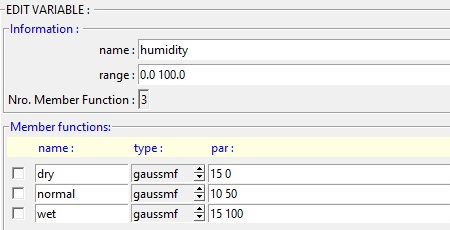
\includegraphics[width=1\linewidth]{pics/info/hum_info}}
    \end{minipage}
    \begin{minipage}[h]{0.5\linewidth}
        \center{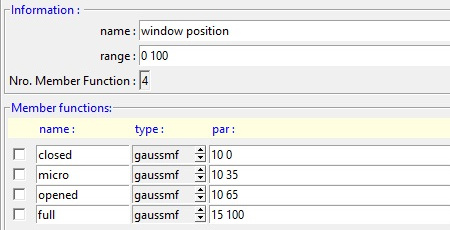
\includegraphics[width=1\linewidth]{pics/info/win_info}}
    \end{minipage}
    \caption{Параметры функций принадлежности} 
\end{figure}

\newpage
По итогу были получены различные графики, которые показывают, как будет
работать система, отрывать и закрываться окно, в зависимости от различных
входных параметров. Примеры на рис. 5, рис. 6, рис. 7. 

\newpage
\begin{figure}[h]
    \center{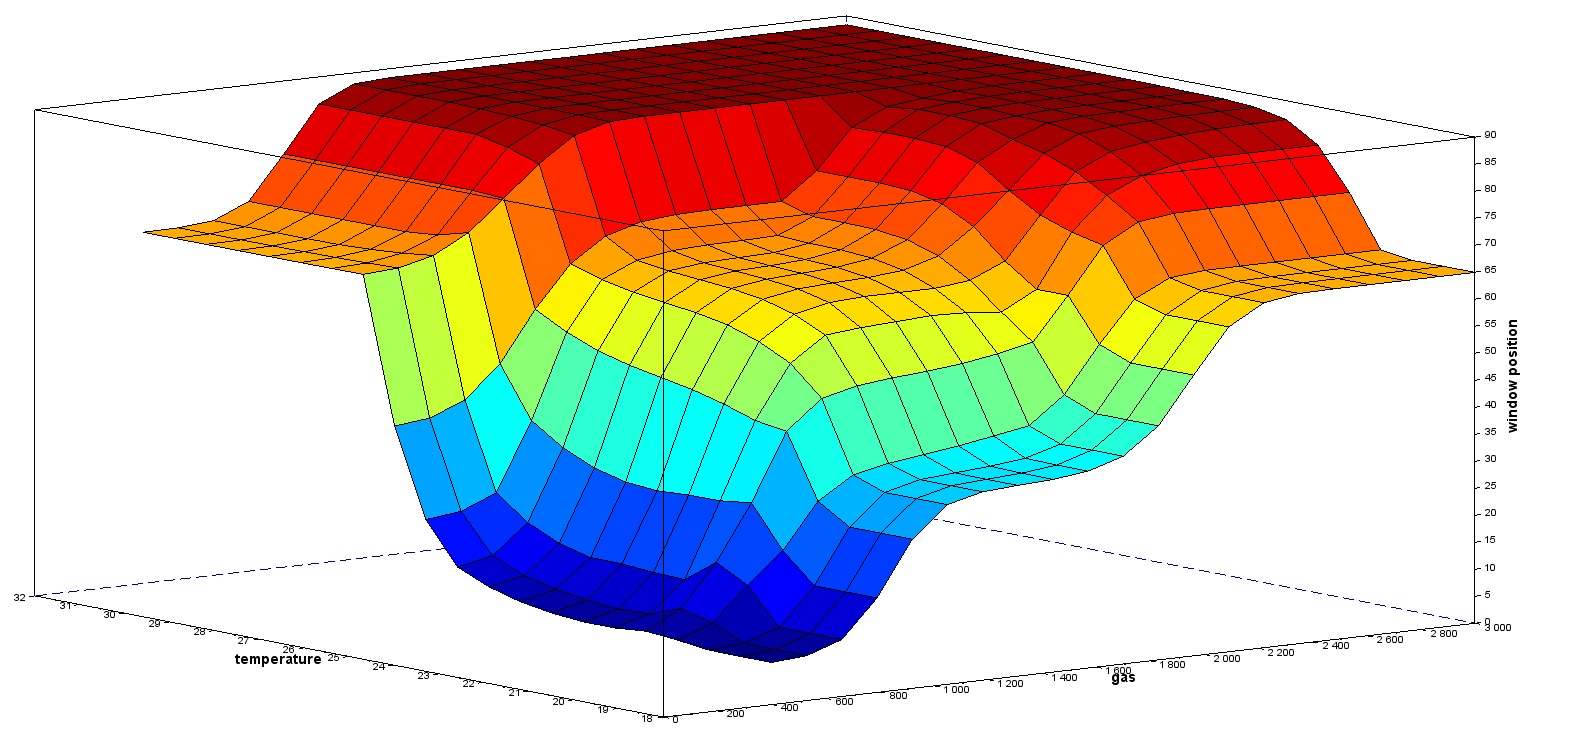
\includegraphics[width=0.55\linewidth]{pics/3d_gas_temp_hum50}}
    \caption{График работы при относительной влажности равной 50\%} 
\end{figure}

\begin{figure}[h]
    \center{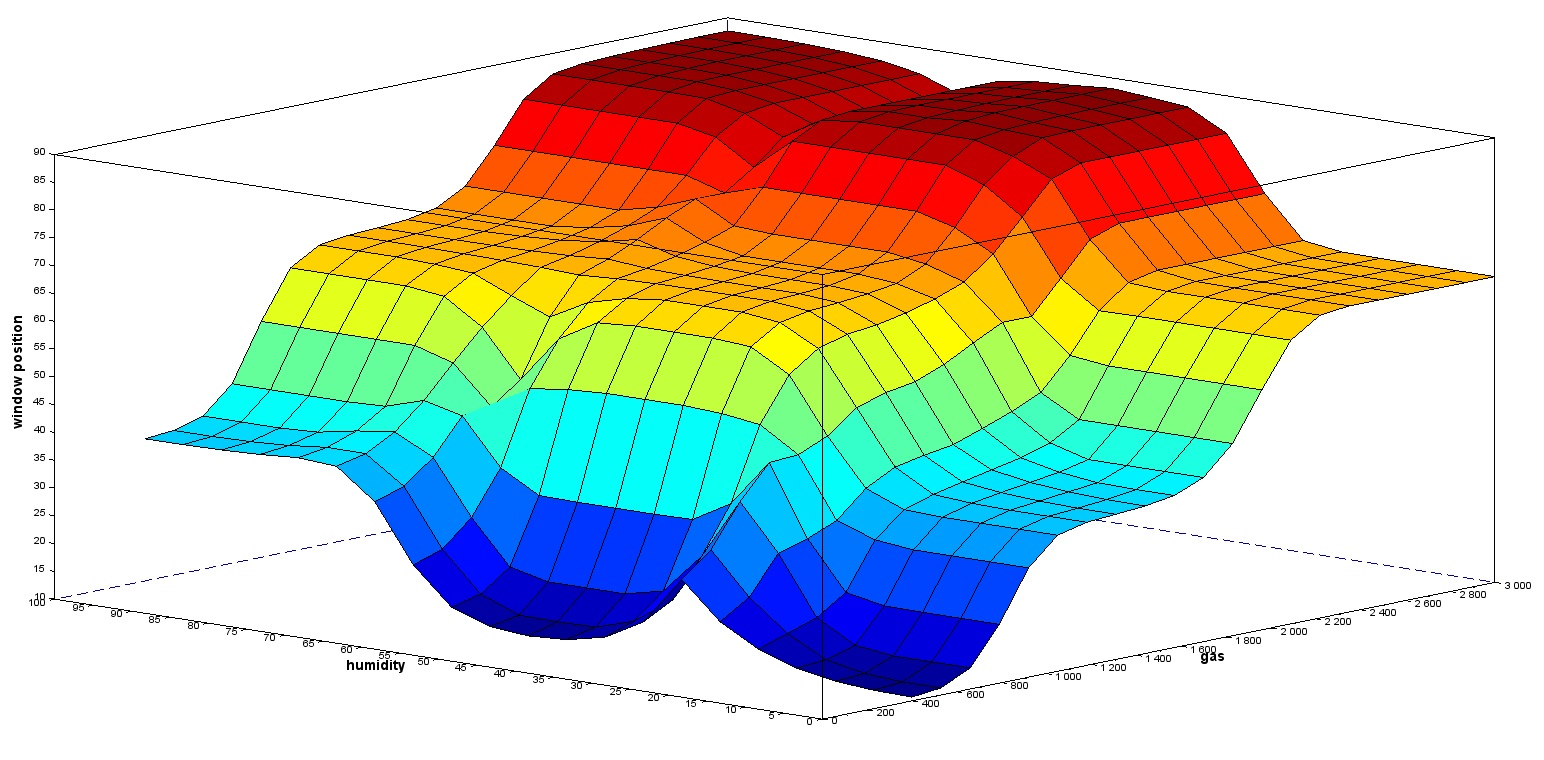
\includegraphics[width=0.55\linewidth]{pics/3d_gas_hum_temp23}}
    \caption{График работы при температуре 23$^{\circ}$C} 
\end{figure}

\begin{figure}[h]
    \center{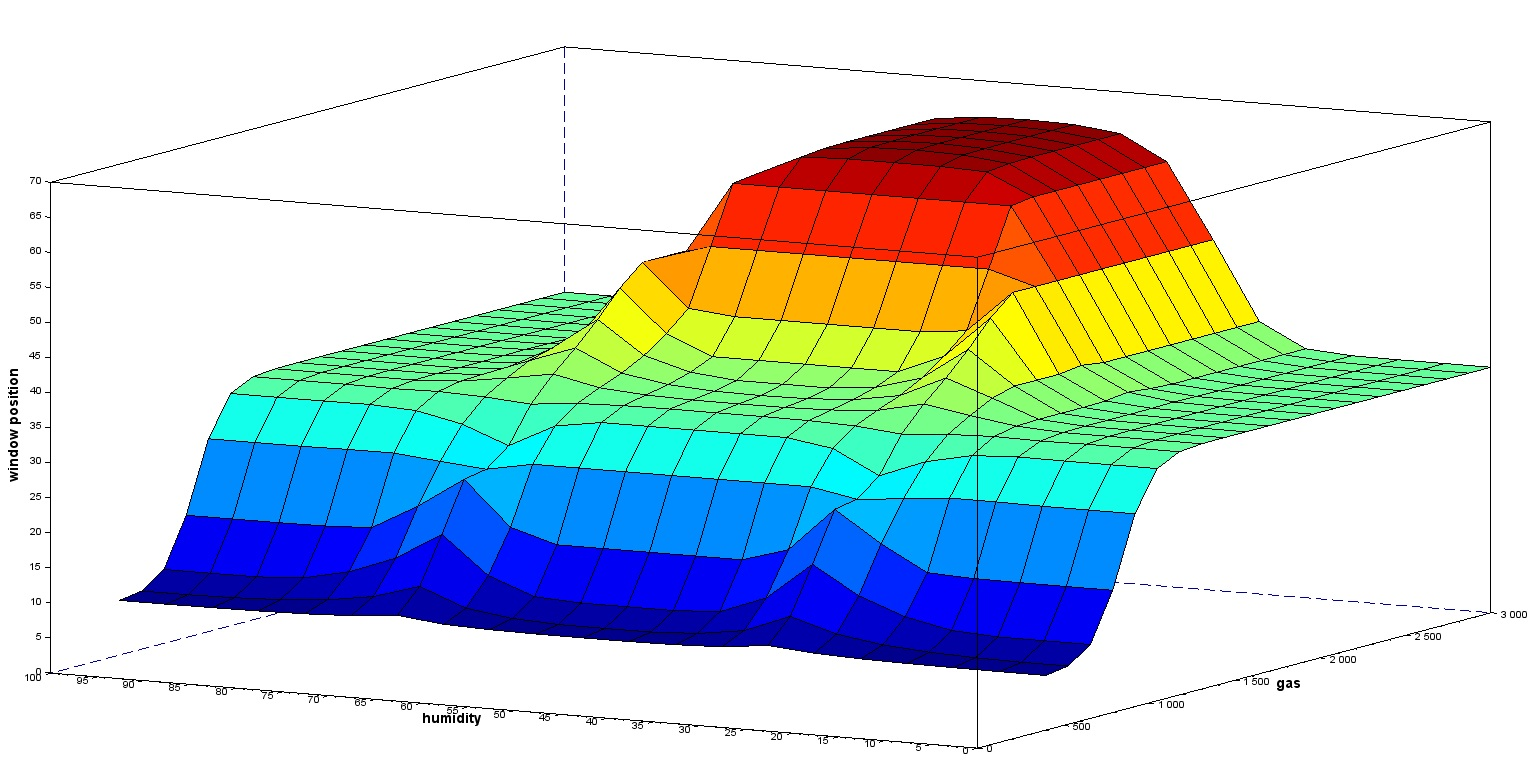
\includegraphics[width=0.55\linewidth]{pics/3d_gas_hum_temp18}}
    \caption{График работы при температуре 18$^{\circ}$C} 
\end{figure}

На двух последних графиках видно, как бы работала система при двух
принципиально разных температурах окружающей среды, холодной и нормальной.

\newpage
\section{Реализация нечёткой логики на МК}
В данном устройстве используются два датчика, дисплей, энекодер и
микроконтроллер. Дисплей и энкодер нужны для вывода и переключения
информации, которую наша система получает или генерирует.

Есть 4 экрана, между которыми можно переключаться: показания температуры,
показания относительной влажности, показания датчика газа и то, насколько
надо открыть окно. Переключение между экранами производится с помощью
абсолютного энкодера.

Датчики опрашиваются один раз в секунду, неблокирующим методом. 
Также каждую секунду решается, насколько надо открыть окно.

Теперь расскажу о реализации алгоритма Мандани.

Сначала произовдится фаззификация переменных. На вход функции приходит
три переменные: температура, влажность и уровень углекислого газа.
Для каждой заводится массив из трёх элементов, в которые записываются
значения функции принадлежности для конкретного терма из терм-множества.

Дальше идёт этап агрегирования подусловий. Для этого заводим 
двумерный массив, в котором у нас будут хранится правила. 
Каждая ячейка массива это одно правило, сохранённое в виде массива: 
[0, 1, 2, 3], где каждая цифра обозначает номер терма из терм-множества.
Первый элемент - уровень углекислого газа, второй - температура,
третий - влажность, четвёртый - как открыто окно.
Для каждого правила вычисляем значение левой части, как минимум из
соответствующих значений функций принадлежности.

Далее идёт этап активизации подзаключений и аккумуляции значений. 
Снова проходим по массиву правил, но теперь смотрим на 
максимальное значение левых частей правила для каждого терма из 
терм-множества состояний окна. Таким образом для каждой из четырёх
функций принадлежности состояний окна находим верхнюю грань, выше 
которой мы значение не рассматриваем.

Потом запускаю цикл от 0 до 100 включительно, с шагом 1, так как
измерение открытия окна идёт в процентах, а это получается дискретное
значение. На каждом шагу цикла смотрим, не превысило ли значение
конкретной функции принадлежности значния, полученног ранее, если превысило,
то мы его ограничиваем, если нет, то сравниваем итоговые значения
четырёх функций принадлежности и выбираем максимальное.

Остаётся только этап дефаззификации с помощью метода центроид.
Вычисляем значение по формуле, для интегрирования используем метод
прямоугольников. Получается не очень точно, но с учётом того, какие у нас
датчики на это можно не обращать внимания.
Таким образом получаем значение, насколько надо открыть окно, чтобы 
сделать в комнате оптимальную атмосферу.

\section{Вывод}
Доделать

\section{Список источников}
Доделать

\end{document}
